% SOURCE: RG_map_evidence_REFIX20260801.json :: cells.*.per_g.{2,3,5,10,20}.median_abs_drop_med3 (low-gain constructive cells; extrema labels computed on g=max subset)
% !TEX encoding = UTF-8 Unicode
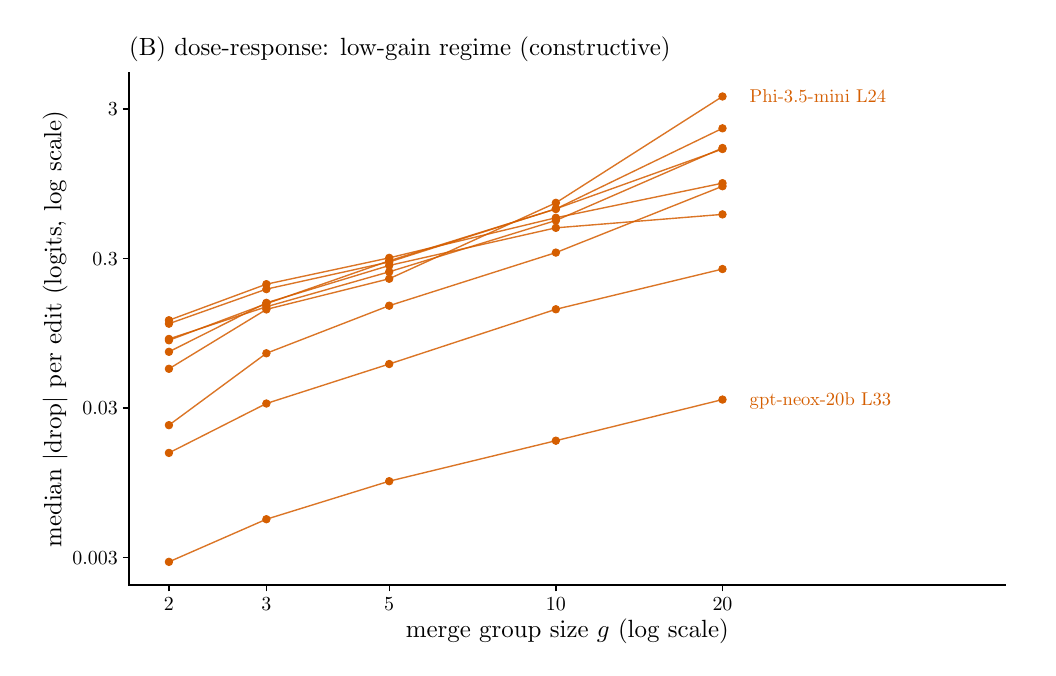
\begin{tikzpicture}[x=1pt,y=1pt]
\definecolor{fillColor}{RGB}{255,255,255}
\path[use as bounding box,fill=fillColor,fill opacity=0.00] (0,0) rectangle (361.35,224.04);
\begin{scope}
\path[clip] (  0.00,  0.00) rectangle (361.35,224.04);
\definecolor{drawColor}{RGB}{255,255,255}
\definecolor{fillColor}{RGB}{255,255,255}

\path[draw=drawColor,line width= 0.5pt,line join=round,line cap=round,fill=fillColor] (  0.00,  0.00) rectangle (361.35,224.04);
\end{scope}
\begin{scope}
\path[clip] ( 36.64, 22.61) rectangle (353.35,207.59);
\definecolor{fillColor}{RGB}{255,255,255}

\path[fill=fillColor] ( 36.64, 22.61) rectangle (353.35,207.59);
\definecolor{drawColor}{RGB}{213,94,0}

\path[draw=drawColor,draw opacity=0.85,line width= 0.5pt,line join=round] ( 51.04, 31.01) --
	( 86.26, 46.42) --
	(130.64, 60.16) --
	(190.86, 74.79) --
	(251.07, 89.65);

\path[draw=drawColor,draw opacity=0.85,line width= 0.5pt,line join=round] ( 51.04,118.32) --
	( 86.26,131.35) --
	(130.64,140.86) --
	(190.86,155.35) --
	(251.07,167.85);

\path[draw=drawColor,draw opacity=0.85,line width= 0.5pt,line join=round] ( 51.04, 70.38) --
	( 86.26, 88.23) --
	(130.64,102.50) --
	(190.86,122.28) --
	(251.07,136.82);

\path[draw=drawColor,draw opacity=0.85,line width= 0.5pt,line join=round] ( 51.04,100.77) --
	( 86.26,122.23) --
	(130.64,133.31) --
	(190.86,160.74) --
	(251.07,199.18);

\path[draw=drawColor,draw opacity=0.85,line width= 0.5pt,line join=round] ( 51.04,111.56) --
	( 86.26,123.19) --
	(130.64,135.82) --
	(190.86,154.36) --
	(251.07,180.55);

\path[draw=drawColor,draw opacity=0.85,line width= 0.5pt,line join=round] ( 51.04, 80.41) --
	( 86.26,106.38) --
	(130.64,123.58) --
	(190.86,142.76) --
	(251.07,166.74);

\path[draw=drawColor,draw opacity=0.85,line width= 0.5pt,line join=round] ( 51.04,106.91) --
	( 86.26,124.61) --
	(130.64,138.11) --
	(190.86,151.71) --
	(251.07,156.57);

\path[draw=drawColor,draw opacity=0.85,line width= 0.5pt,line join=round] ( 51.04,111.07) --
	( 86.26,124.30) --
	(130.64,139.80) --
	(190.86,158.54) --
	(251.07,187.67);

\path[draw=drawColor,draw opacity=0.85,line width= 0.5pt,line join=round] ( 51.04,117.07) --
	( 86.26,129.56) --
	(130.64,139.38) --
	(190.86,158.58) --
	(251.07,180.18);
\definecolor{drawColor}{RGB}{213,94,0}
\definecolor{fillColor}{RGB}{213,94,0}

\path[draw=drawColor,line width= 0.3pt,line join=round,line cap=round,fill=fillColor] ( 51.04,100.77) circle (  1.36);

\path[draw=drawColor,line width= 0.3pt,line join=round,line cap=round,fill=fillColor] ( 86.26,122.23) circle (  1.36);

\path[draw=drawColor,line width= 0.3pt,line join=round,line cap=round,fill=fillColor] (130.64,133.31) circle (  1.36);

\path[draw=drawColor,line width= 0.3pt,line join=round,line cap=round,fill=fillColor] (190.86,160.74) circle (  1.36);

\path[draw=drawColor,line width= 0.3pt,line join=round,line cap=round,fill=fillColor] (251.07,199.18) circle (  1.36);

\path[draw=drawColor,line width= 0.3pt,line join=round,line cap=round,fill=fillColor] ( 51.04,111.56) circle (  1.36);

\path[draw=drawColor,line width= 0.3pt,line join=round,line cap=round,fill=fillColor] ( 86.26,123.19) circle (  1.36);

\path[draw=drawColor,line width= 0.3pt,line join=round,line cap=round,fill=fillColor] (130.64,135.82) circle (  1.36);

\path[draw=drawColor,line width= 0.3pt,line join=round,line cap=round,fill=fillColor] (190.86,154.36) circle (  1.36);

\path[draw=drawColor,line width= 0.3pt,line join=round,line cap=round,fill=fillColor] (251.07,180.55) circle (  1.36);

\path[draw=drawColor,line width= 0.3pt,line join=round,line cap=round,fill=fillColor] ( 51.04, 80.41) circle (  1.36);

\path[draw=drawColor,line width= 0.3pt,line join=round,line cap=round,fill=fillColor] ( 86.26,106.38) circle (  1.36);

\path[draw=drawColor,line width= 0.3pt,line join=round,line cap=round,fill=fillColor] (130.64,123.58) circle (  1.36);

\path[draw=drawColor,line width= 0.3pt,line join=round,line cap=round,fill=fillColor] (190.86,142.76) circle (  1.36);

\path[draw=drawColor,line width= 0.3pt,line join=round,line cap=round,fill=fillColor] (251.07,166.74) circle (  1.36);

\path[draw=drawColor,line width= 0.3pt,line join=round,line cap=round,fill=fillColor] ( 51.04,106.91) circle (  1.36);

\path[draw=drawColor,line width= 0.3pt,line join=round,line cap=round,fill=fillColor] ( 86.26,124.61) circle (  1.36);

\path[draw=drawColor,line width= 0.3pt,line join=round,line cap=round,fill=fillColor] (130.64,138.11) circle (  1.36);

\path[draw=drawColor,line width= 0.3pt,line join=round,line cap=round,fill=fillColor] (190.86,151.71) circle (  1.36);

\path[draw=drawColor,line width= 0.3pt,line join=round,line cap=round,fill=fillColor] (251.07,156.57) circle (  1.36);

\path[draw=drawColor,line width= 0.3pt,line join=round,line cap=round,fill=fillColor] ( 51.04,111.07) circle (  1.36);

\path[draw=drawColor,line width= 0.3pt,line join=round,line cap=round,fill=fillColor] ( 86.26,124.30) circle (  1.36);

\path[draw=drawColor,line width= 0.3pt,line join=round,line cap=round,fill=fillColor] (130.64,139.80) circle (  1.36);

\path[draw=drawColor,line width= 0.3pt,line join=round,line cap=round,fill=fillColor] (190.86,158.54) circle (  1.36);

\path[draw=drawColor,line width= 0.3pt,line join=round,line cap=round,fill=fillColor] (251.07,187.67) circle (  1.36);

\path[draw=drawColor,line width= 0.3pt,line join=round,line cap=round,fill=fillColor] ( 51.04,117.07) circle (  1.36);

\path[draw=drawColor,line width= 0.3pt,line join=round,line cap=round,fill=fillColor] ( 86.26,129.56) circle (  1.36);

\path[draw=drawColor,line width= 0.3pt,line join=round,line cap=round,fill=fillColor] (130.64,139.38) circle (  1.36);

\path[draw=drawColor,line width= 0.3pt,line join=round,line cap=round,fill=fillColor] (190.86,158.58) circle (  1.36);

\path[draw=drawColor,line width= 0.3pt,line join=round,line cap=round,fill=fillColor] (251.07,180.18) circle (  1.36);

\path[draw=drawColor,line width= 0.3pt,line join=round,line cap=round,fill=fillColor] ( 51.04, 31.01) circle (  1.36);

\path[draw=drawColor,line width= 0.3pt,line join=round,line cap=round,fill=fillColor] ( 86.26, 46.42) circle (  1.36);

\path[draw=drawColor,line width= 0.3pt,line join=round,line cap=round,fill=fillColor] (130.64, 60.16) circle (  1.36);

\path[draw=drawColor,line width= 0.3pt,line join=round,line cap=round,fill=fillColor] (190.86, 74.79) circle (  1.36);

\path[draw=drawColor,line width= 0.3pt,line join=round,line cap=round,fill=fillColor] (251.07, 89.65) circle (  1.36);

\path[draw=drawColor,line width= 0.3pt,line join=round,line cap=round,fill=fillColor] ( 51.04,118.32) circle (  1.36);

\path[draw=drawColor,line width= 0.3pt,line join=round,line cap=round,fill=fillColor] ( 86.26,131.35) circle (  1.36);

\path[draw=drawColor,line width= 0.3pt,line join=round,line cap=round,fill=fillColor] (130.64,140.86) circle (  1.36);

\path[draw=drawColor,line width= 0.3pt,line join=round,line cap=round,fill=fillColor] (190.86,155.35) circle (  1.36);

\path[draw=drawColor,line width= 0.3pt,line join=round,line cap=round,fill=fillColor] (251.07,167.85) circle (  1.36);

\path[draw=drawColor,line width= 0.3pt,line join=round,line cap=round,fill=fillColor] ( 51.04, 70.38) circle (  1.36);

\path[draw=drawColor,line width= 0.3pt,line join=round,line cap=round,fill=fillColor] ( 86.26, 88.23) circle (  1.36);

\path[draw=drawColor,line width= 0.3pt,line join=round,line cap=round,fill=fillColor] (130.64,102.50) circle (  1.36);

\path[draw=drawColor,line width= 0.3pt,line join=round,line cap=round,fill=fillColor] (190.86,122.28) circle (  1.36);

\path[draw=drawColor,line width= 0.3pt,line join=round,line cap=round,fill=fillColor] (251.07,136.82) circle (  1.36);

\node[text=drawColor,anchor=base west,inner sep=0pt, outer sep=0pt, scale=  0.67] at (260.92,196.88) {Phi-3.5-mini L24};

\node[text=drawColor,anchor=base west,inner sep=0pt, outer sep=0pt, scale=  0.67] at (260.92, 87.34) {gpt-neox-20b L33};
\end{scope}
\begin{scope}
\path[clip] (  0.00,  0.00) rectangle (361.35,224.04);
\definecolor{drawColor}{RGB}{0,0,0}

\path[draw=drawColor,line width= 0.5pt,line join=round,line cap=rect] ( 36.64, 22.61) --
	( 36.64,207.59);
\end{scope}
\begin{scope}
\path[clip] (  0.00,  0.00) rectangle (361.35,224.04);
\definecolor{drawColor}{RGB}{0,0,0}

\node[text=drawColor,anchor=base east,inner sep=0pt, outer sep=0pt, scale=  0.72] at ( 32.59, 30.15) {0.003};

\node[text=drawColor,anchor=base east,inner sep=0pt, outer sep=0pt, scale=  0.72] at ( 32.59, 84.16) {0.03};

\node[text=drawColor,anchor=base east,inner sep=0pt, outer sep=0pt, scale=  0.72] at ( 32.59,138.17) {0.3};

\node[text=drawColor,anchor=base east,inner sep=0pt, outer sep=0pt, scale=  0.72] at ( 32.59,192.18) {3};
\end{scope}
\begin{scope}
\path[clip] (  0.00,  0.00) rectangle (361.35,224.04);
\definecolor{drawColor}{RGB}{0,0,0}

\path[draw=drawColor,line width= 0.5pt,line join=round] ( 34.39, 32.63) --
	( 36.64, 32.63);

\path[draw=drawColor,line width= 0.5pt,line join=round] ( 34.39, 86.64) --
	( 36.64, 86.64);

\path[draw=drawColor,line width= 0.5pt,line join=round] ( 34.39,140.65) --
	( 36.64,140.65);

\path[draw=drawColor,line width= 0.5pt,line join=round] ( 34.39,194.66) --
	( 36.64,194.66);
\end{scope}
\begin{scope}
\path[clip] (  0.00,  0.00) rectangle (361.35,224.04);
\definecolor{drawColor}{RGB}{0,0,0}

\path[draw=drawColor,line width= 0.5pt,line join=round,line cap=rect] ( 36.64, 22.61) --
	(353.35, 22.61);
\end{scope}
\begin{scope}
\path[clip] (  0.00,  0.00) rectangle (361.35,224.04);
\definecolor{drawColor}{RGB}{0,0,0}

\path[draw=drawColor,line width= 0.5pt,line join=round] ( 51.04, 20.36) --
	( 51.04, 22.61);

\path[draw=drawColor,line width= 0.5pt,line join=round] ( 86.26, 20.36) --
	( 86.26, 22.61);

\path[draw=drawColor,line width= 0.5pt,line join=round] (130.64, 20.36) --
	(130.64, 22.61);

\path[draw=drawColor,line width= 0.5pt,line join=round] (190.86, 20.36) --
	(190.86, 22.61);

\path[draw=drawColor,line width= 0.5pt,line join=round] (251.07, 20.36) --
	(251.07, 22.61);
\end{scope}
\begin{scope}
\path[clip] (  0.00,  0.00) rectangle (361.35,224.04);
\definecolor{drawColor}{RGB}{0,0,0}

\node[text=drawColor,anchor=base,inner sep=0pt, outer sep=0pt, scale=  0.72] at ( 51.04, 13.60) {2};

\node[text=drawColor,anchor=base,inner sep=0pt, outer sep=0pt, scale=  0.72] at ( 86.26, 13.60) {3};

\node[text=drawColor,anchor=base,inner sep=0pt, outer sep=0pt, scale=  0.72] at (130.64, 13.60) {5};

\node[text=drawColor,anchor=base,inner sep=0pt, outer sep=0pt, scale=  0.72] at (190.86, 13.60) {10};

\node[text=drawColor,anchor=base,inner sep=0pt, outer sep=0pt, scale=  0.72] at (251.07, 13.60) {20};
\end{scope}
\begin{scope}
\path[clip] (  0.00,  0.00) rectangle (361.35,224.04);
\definecolor{drawColor}{RGB}{0,0,0}

\node[text=drawColor,anchor=base,inner sep=0pt, outer sep=0pt, scale=  0.90] at (195.00,  3.75) {merge group size $g$ (log scale)};
\end{scope}
\begin{scope}
\path[clip] (  0.00,  0.00) rectangle (361.35,224.04);
\definecolor{drawColor}{RGB}{0,0,0}

\node[text=drawColor,rotate= 90.00,anchor=base,inner sep=0pt, outer sep=0pt, scale=  0.90] at ( 12.20,115.10) {median $|$drop$|$ per edit (logits, log scale)};
\end{scope}
\begin{scope}
\path[clip] (  0.00,  0.00) rectangle (361.35,224.04);
\definecolor{drawColor}{RGB}{0,0,0}

\node[text=drawColor,anchor=base west,inner sep=0pt, outer sep=0pt, scale=  0.90] at ( 36.64,213.84) {(B) dose-response: low-gain regime (constructive)};
\end{scope}
\end{tikzpicture}
